\subsection{\eu Architecture}
\label{sec:europa:arch}

The following figure displays the main architectural components in EUROPA and their relationships:


\begin{figure}
\centering
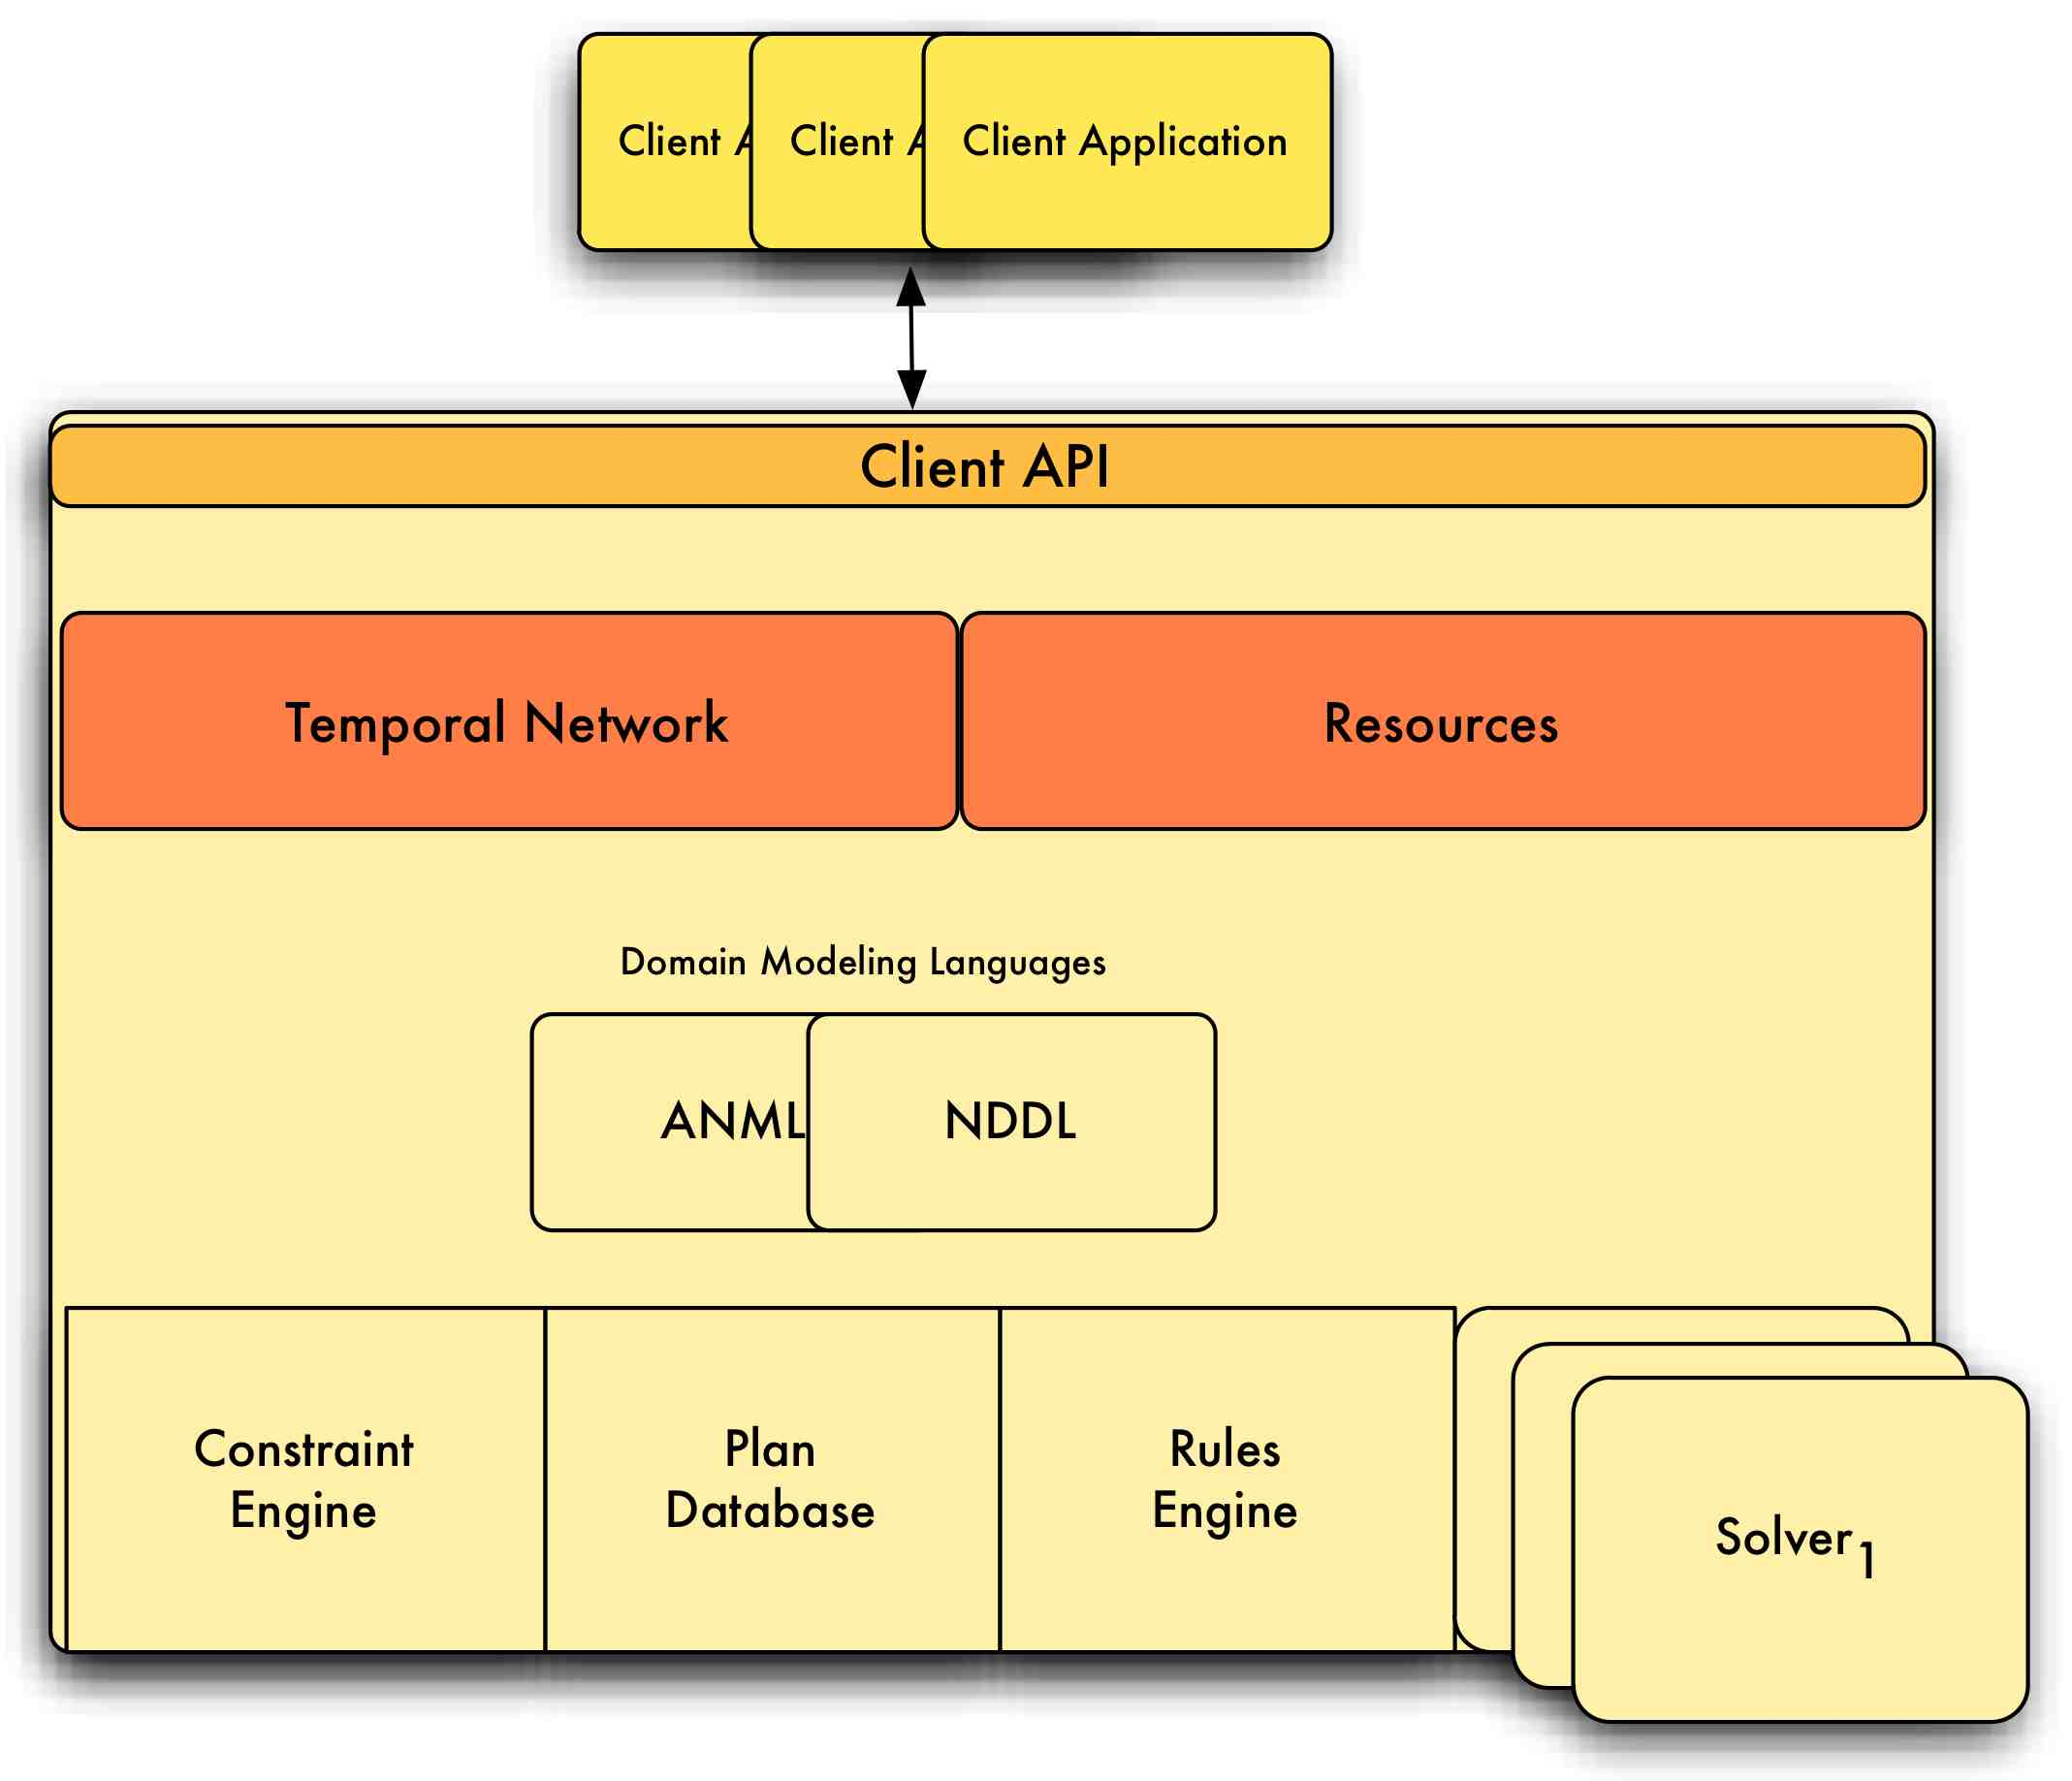
\includegraphics[scale=0.5]{figs/EUROPA-Architecture.jpg}
\caption{\small EUROPA's Architecture}
\label{fig:europa-architecture}
\vskip+0.1cm
\end{figure}


\begin{enumerate}

	\item The Constraint Reasoning Engine (CRE): manages variables, the domains from which they can take values, and constraints that define relationships among variables. It also provides an efficient arc consistency mechanism (TODO: ref to AC-3). The CRE is designed so that specialized reasoning algorithms for specific constraints can be easily and efficiently plugged in.

	\item The Plan Database (PDB): manages object types and objects, which are a mechanism to group variables to more naturally model the real world in much the same way that object oriented programming does. Also manages tokens, which are a mechanism to group variables to represent temporally scoped state. Objects and tokens can be used to model planning domains in a much more natural and extensible way that a pure CSP approach can.

	\item The Rules Engine (RE): manages token relationships in a planning model

	\item The language modules: NDDL, ANML, and other higher level modeling languages can me used to create domain models and problem instances (TODO: point advantages over pure programming API approaches, provide snippets)

	\item API Layer: makes all the services available so that EUROPA can be used to build applications.

\begin{figure}
\centering
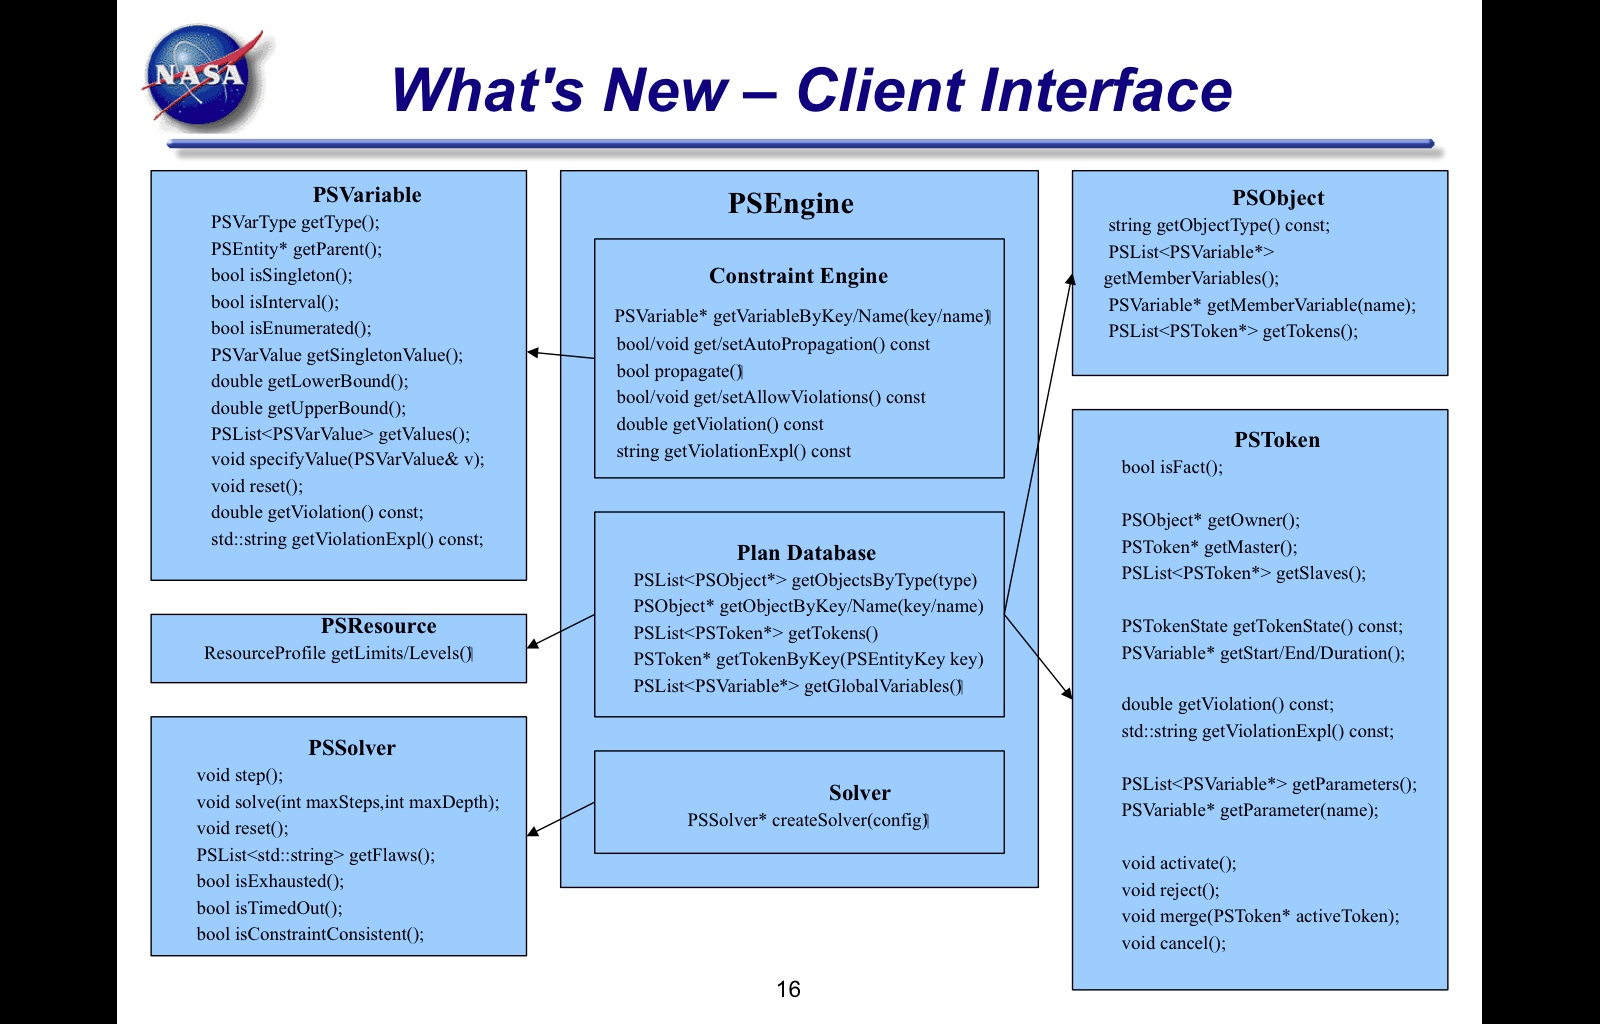
\includegraphics[scale=0.35]{figs/EUROPA-API.jpg}
\caption{\small EUROPA's Client API}
\label{fig:europa-api}
\vskip+0.1cm
\end{figure}


	\item Extension Modules bundled with EUROPA: Temporal Network, Resources, NDDL, ANML.
		\begin{enumerate}
			\item Temporal Network
			\item Resources
			\item NDDL
			\item ANML (TODO:maybe it's better to leave out?)
		\end{enumerate}

\end{enumerate}


\subsection{Modeling}
\label{sec:europa:modeling}

EUROPA can ingest descriptions of models, plans and goals. This means that a single planner can be applied to different systems and problems, simply by providing different models and goals. For such planners the expressiveness of the languages for models, goals and plans is of great importance. EUROPA provides a high level language called NDDL (New Domain Description Language) that allows the user to specify the different components of a problem domain in a concise way. The main characteristics that make NDDL a powerful tool for describing problem domains are:

\begin{enumerate}
	\item It's Object Oriented: NDDL supports classes and inheritance in similar fashion to popular Object-Oriented languages like Java and C++. It also supports polymorphism for some of the planning components. Using object classes and instances is a time-tested approach to naturally describe problem domains (TODO: OO ref?).
	\item It offers declarative constructs to define constraints and causality dependencies between actions and effects.
	\item It offers procedural constructs to populate EUROPA's plan database with specific problem instances expressed in terms of objects, variables, constraints, facts and goals.
\end{enumerate}

To understand how the most important elements of NDDL work, let's take a look at how the Shopping Agent problem described above would be modeled:

\begin{verbatim}

// Locations (Home, SuperMarket, etc.)
class Location {
  string name;
  Location(string _name){
    name = _name;
  }
}

// Products (Milk, Banana, etc.) and
class Product {
  string name;
  Product(string _name) {
    name = _name;
  }
}

// ProductLocations (Banana can be found at SuperMarket, for example)
class ProductLocation {
  Location location;
  Product product;

  ProductLocation(Location _location, Product _product){
    location = _location;
    product = _product;
  }
}

// Use built-in Timeline functionality to enforce that an agent:
// a) Can't be at more than one place at a time.
// b) Can't Go more than one place at a time.
// c) Can't Go somewhere and be At somewhere at the same time.
class AgentLocation extends Timeline{
  predicate At {
    Location loc;
  }

  predicate Going {
    Location from;
    Location to;
  }
}

// In addition to having a location timeline, the agent can buy and own things.  
// Note that the actions and the location predicates can be concurrent 
// so they can't be on the same Timeline
class Agent {
  AgentLocation location;

  Agent() {
    location = new AgentLocation();
  }

  action Buy {
    Product product;
  }
  
  action Go {
    Location from;
    Location to;
  }
  
  predicate Own {
  	Product product;
  }
}


// Define the rules for our actions:
Agent::Go {
  met_by(condition object.location.At origin);
  eq(from, origin.loc);
 
  equals(effect object.location.Going going);
  eq(going.from, from);
  eq(going.to, to);
   
  meets(effect object.location.At destination);
  eq(to, destination.loc);
}

Agent::Buy {
  // A Buy takes 10 time units
  eq(10, duration);

  // initialized to all locations
  ProductLocation possibleStores;

  // limit possibleStores variables to ones that provide what we need to buy
  eq(product, possibleStores.product);

  // We must be At a location during our Buy, and that location must have the
  // product we want available:
  contained_by(condition object.location.At currLocation);
  eq(currLocation.loc, possibleStores.location);
  
  starts(effect Own purchase);
  eq(purchase.product,product);
}

\end{verbatim}


In this model we can see:

TODO: explain variable, object, predicate and action types, including constraints that can be part of them
\begin{enumerate}
	\item Variable Types: This model uses integer (activity duration, start and end times, etc) and string (Location and Product names, etc)
	\item Object Types:
	\item Predicate Types:
	\item Action Types:
\end{enumerate}


Now let's look at how a specific problem instance would be specified in NDDL:

\begin{verbatim}

// Allocate instances
Location Home = new Location("Home");
Location SuperMarket = new Location("SuperMarket");
Location HardwareStore = new Location("HardwareStore");

Product Banana = new Product("Banana");
Product Milk = new Product("Milk");
Product Drill = new Product("Drill");

ProductLocation bananaLocation = new ProductLocation(SuperMarket, Banana);
ProductLocation milkLocation = new ProductLocation(SuperMarket, Milk);
ProductLocation drillLocation = new ProductLocation(HardwareStore, Drill);

Agent agent = new Agent();

// Indicate that the database is closed - no new objects can be created
// this allows EUROPA to perform more efficient inference
close();

// We start the day at Home:
fact(agent.location.At atHomeForBreakfast);
atHomeForBreakfast.loc.specify(Home);

// Goals for all of the agent's needs, buy if needed
goal(agent.Own gotMilk);
gotMilk.product.specify(Milk);
goal(agent.Own gotBanana);
gotBanana.product.specify(Banana);
goal(agent.Own gotDrill);
gotDrill.product.specify(Drill);

// Make sure agent is home for dinner
goal(agent.location.At atHomeForDinner);
atHomeForDinner.loc.specify(Home);

// Agent has all day to satisfy goals:
gotMilk after atHomeForBreakfast;
gotMilk before atHomeForDinner;

gotBanana after atHomeForBreakfast;
gotBanana before atHomeForDinner;

gotDrill after atHomeForBreakfast;
gotDrill before atHomeForDinner;

// Force things to happen within our planning horizon:
int horizonStart = 0;
int horizonEnd = 100;
leq(horizonStart, atHomeForBreakfast.start);
leq(atHomeForDinner.end, horizonEnd);

\end{verbatim}

TODO:  explain variable, object, predicate and constraint instances.
explain goals and facts.

\begin{enumerate}
	\item Variable Instances:
	\item Object Instances:
	\item Facts:
	\item Goals:
	\item Constraint Instances:
\end{enumerate}


\subsection{Inference}
\label{sec:europa:inference}

TODO: explain how inference is used to detect perform bounds propagation, domain reduction and to detect constraint violations.
- talk about AC3 implementation and extension mechanisms
- talk about europa's constraint library


The Temporal Network:
The notion of time is central to temporal planning. EUROPA uses variables to explicitly represent timepoints for plan activities and states. Constraints among timepoints provide a natural way to express domain axioms. For example, in order to state that activity A must occur before activity B we can say that the end timepoint of A is <= the start timepoint of B. 

\begin{figure}
\centering
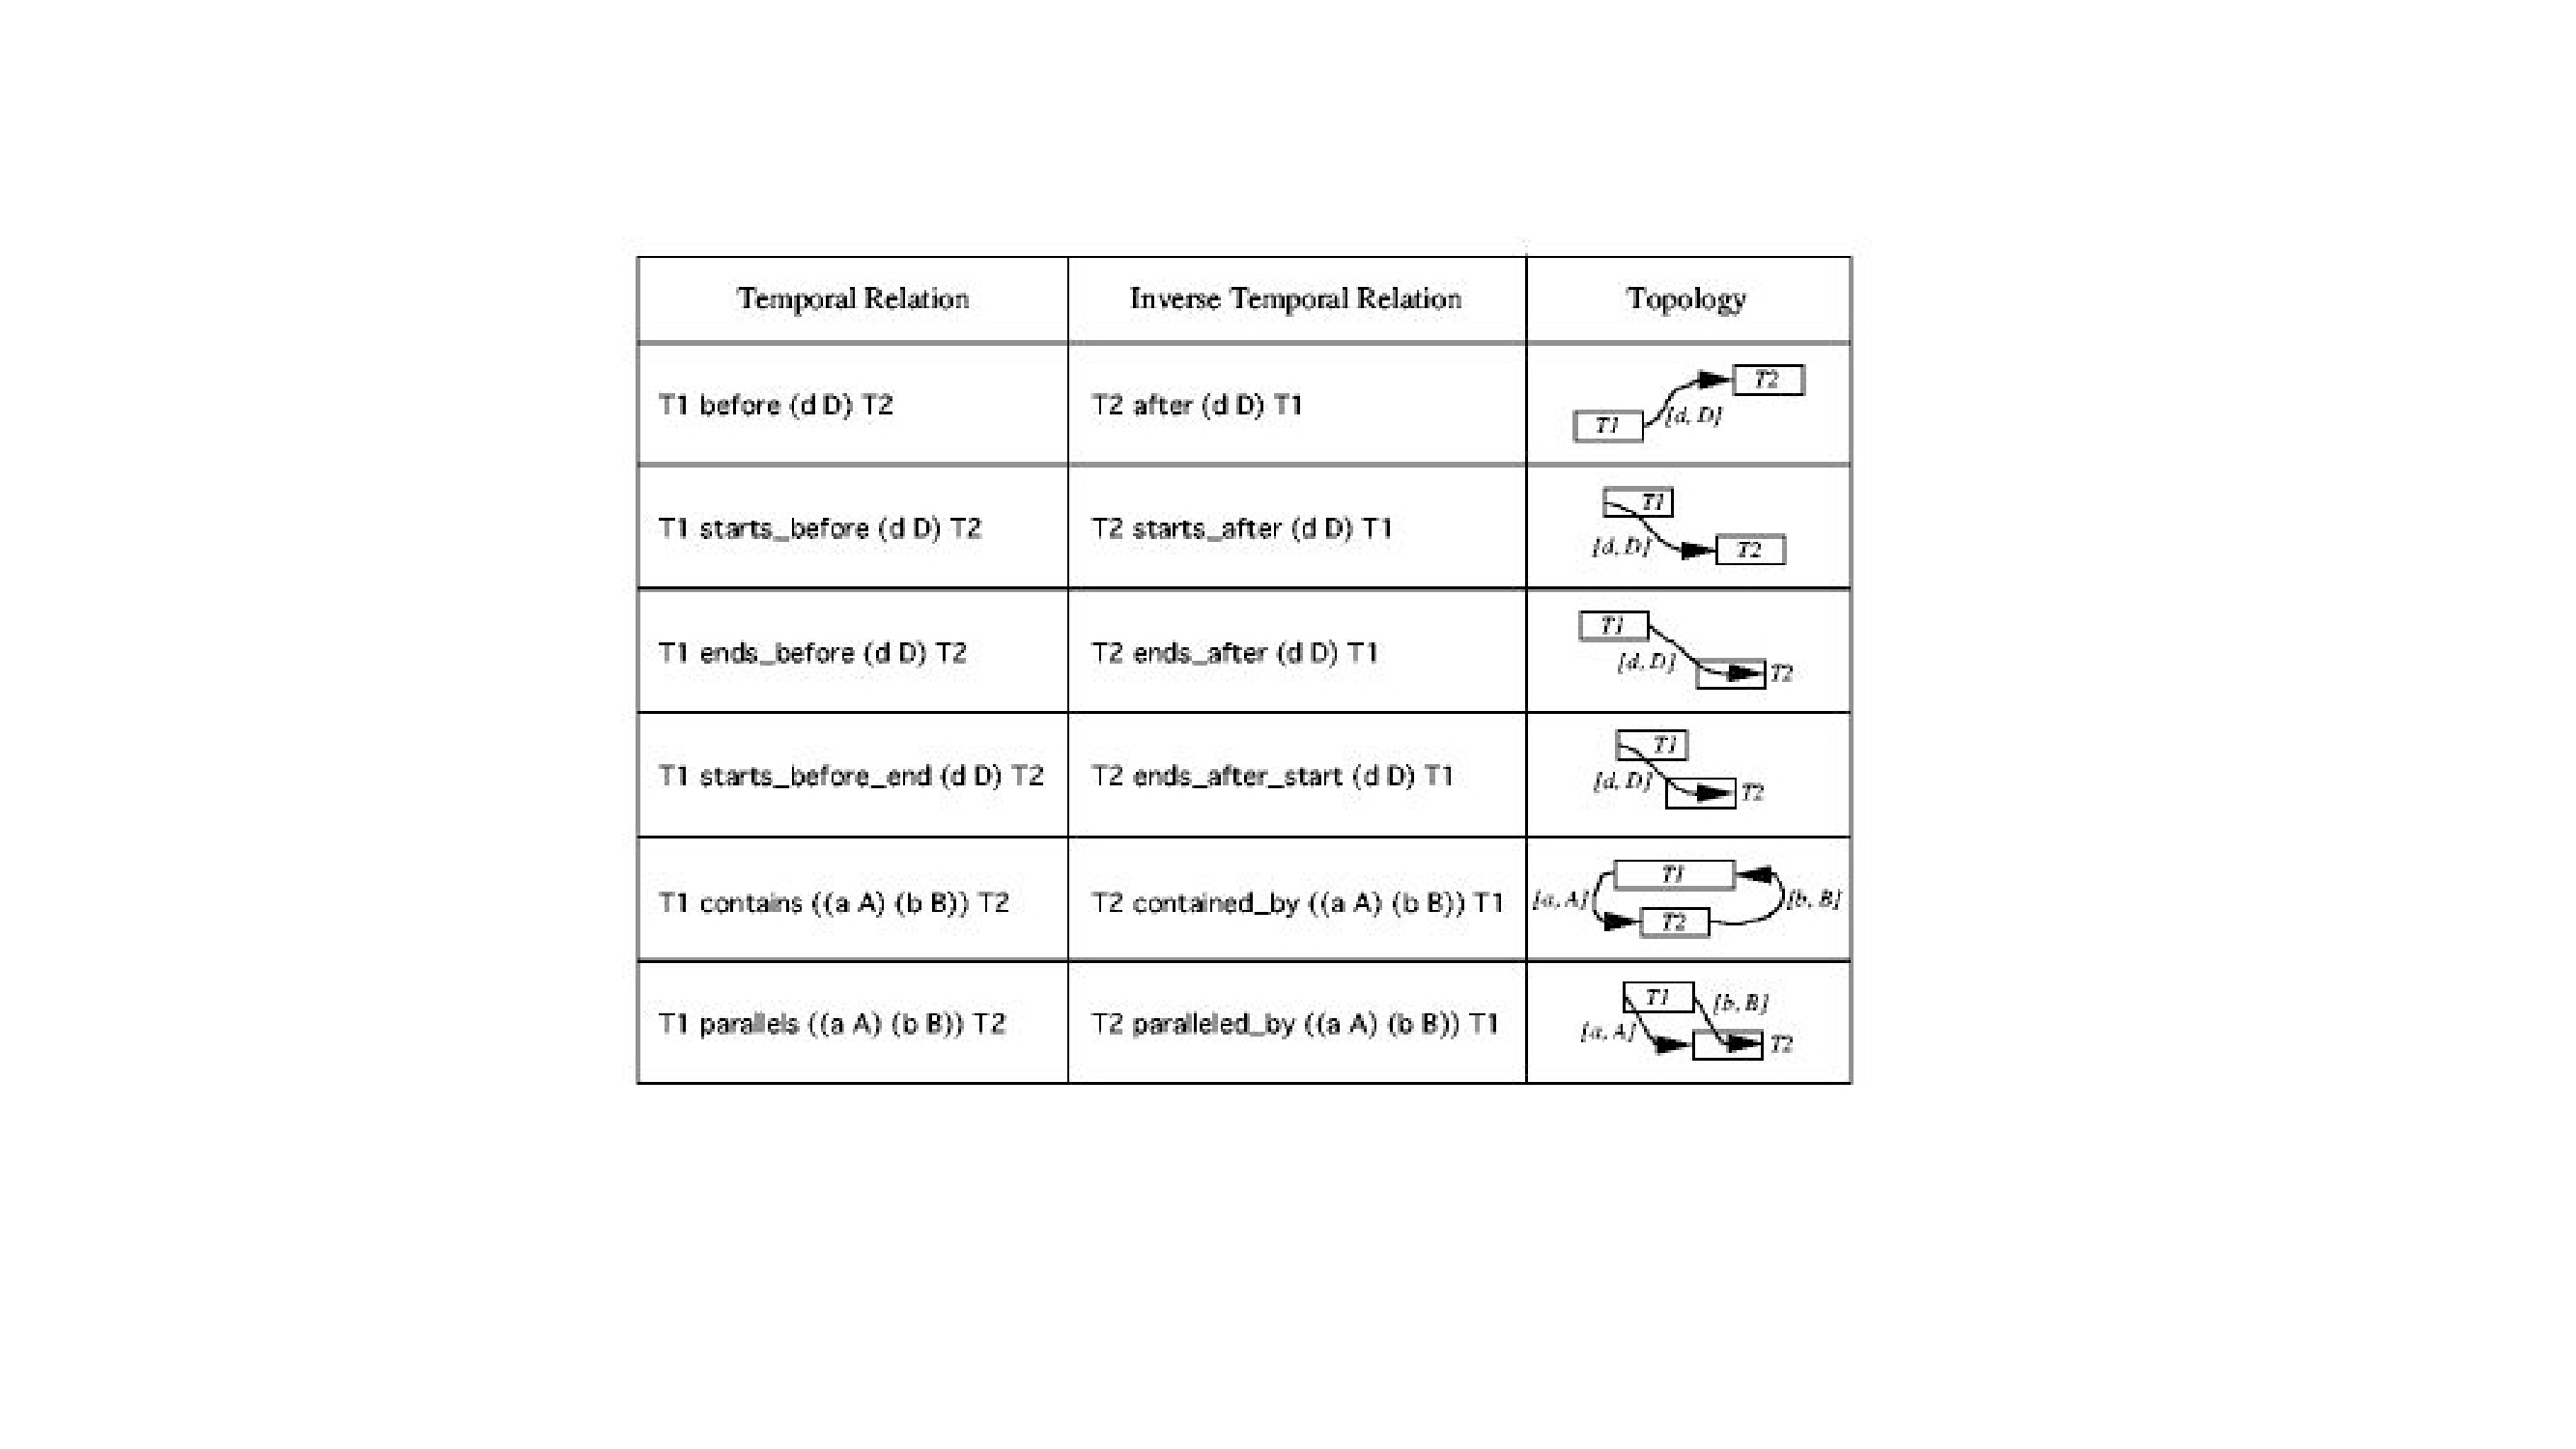
\includegraphics[scale=0.3]{figs/Allen-algebra.pdf}
\caption{\small Temporal relations defined within the planner are
  based on \texttt{Allen Algebra} relations shown above.}
\label{fig:allen-algebra}
\vskip-0.3cm
\end{figure}

Dechter et al. (Dechter 1991) proposed that constraints among timepoints can be grouped together to form a Simple Temporal Network (STN). Such a network can be transformed into a Distance Graph (DG) where the outward arc from a node represents the maximum distance from the source node to the target node. The diagram below illustrates a simple STN with just 2 variables and a single constraint. It also shows the resulting DG. 

TODO: add figure

Dechter et al. (Dechter 1991) also showed that shortest path algorithms could be used to propagate values in the network and discover a negative cycle. A negative cycle is a path from a node to itself that has a path length less than 0. If such a cycle exists, the network is inconsistent. It was further shown that a single-source shortest path algorithm was sufficient to detect a negative cycle and provide sufficient propagation to yield a backtrack-free search. Thus we have an efficient and complete algorithm for propagating an STN. These results build on the already established notion of a CSP and are naturally incorporated into the general representation and propagation scheme used in EUROPA. 

Resources:

    Reservoir resources can have both 'consume' and 'produce' tokens. Note that these tokens do NOT have the usual start/end/duration token variables, since occur at a single instant in time. Instead, they have a single variable, 'time' used to represent that instant.
    Reusable resources have 'uses' tokens that use a quantity for the duration of the token. These tokens do have the usual start/end/duration variables.
    Unary resources are reusable resources with unit quantity and have 'use' tokens (again, with the usual start/end/duration variables). 
    
    TODO: talk about resource envelope computation by using MaxFlow formulation.


\subsection{Search}
\label{sec:europa:search}

Now we have all the elements in place so that an automated problem solver can be created. Let's recap what those elements are:

\begin{enumerate}

\item A domain model that describes the variable, object, predicate and action types that are relevant for the problem.
\item A problem instance (also called initial state) that consists of:
	\item Variable and Object instances that exist for the entire planning horizon.
	\item Temporally scoped predicate and action instances.
	\item Temporally scoped goals.

\end{enumerate}
	
All this information is kept in EUROPA's  Plan Database so that inference and search mechanisms can be used to look for a problem solution.

Given that temporal intervals may extend indefinitely in both positive and negative directions, for problems with a temporal dimension it is also common to specify a Planning Horizon when invoking a solver. The Planning Horizon is the temporal interval that a problem solver has to worry about, any decisions that fall completely outside of the Planning Horizon can be ignored. This is very useful for recurrent activities, consider for instance a model where a medical checkup has to occur every 3 months, the user can model a recurring activity and then use the Planning Horizon to ensure that a finite number of medical checkup activities are generated as part of a plan. This is also useful to ignore activities that may happen too far in the future or in the past to be relevant for a particular plan, this way the user can ensure that the solver is making as few commitments as necessary.

EUROPA provides a built-in solver that performs Plan Space Planning (TODO: ref), in this approach, the initial state is considered a partial plan that needs to be refined toward a solution plan that achieves the goals. The operations to refine the partial plan PP at any time are:
\begin{enumerate}
	\item Find the flaws of PP, that is the conditions that prevent it from being a solution plan (flaw types are explained below).
	\item Select one such flaw
	\item Select a resolver for the flaw
	\item Refine PP by applying the resolver
	\item If an inconsistency is found, try another resolver.
	\item If all possible resolvers for a particular flaw fail, return failure, otherwise continue until resolving all the flaws.
\end{enumerate}
	
This Plan Space Planning algorithm is translated into EUROPA's representation as follows:

The initial partial plan is the state of EUROPA's Plan Database after the initial state has been instantiated, this results in a set of variable, object and token instances. Inference then takes place to detect flaws in the partial plan, there are 3 kinds of flaws that can be detected:

\begin{enumerate}
	\item Unbound Variable: a variable in the partial plan whose domain is not a singleton. Unbound Variables are resolved by specification of a value from the domain of the variable.

	\item Open Condition: an open condition is an inactive token. Inactive tokens can be generated by explicitly posted goals, or when a token is activated, rules may fire that create inactive slave tokens (TODO: point to more detailed decription above in Rules Engine section).  Open Conditions can be resolved in three ways: 
\begin{enumerate}
		\item Merging: A free activity is merged with a matching activity already in the plan. An activity a is said to match an activity a? if a and a? unify and the temporal constraints involving a are satis�ed by a?. Thus,  a and a? can be considered the same activity and we do not need to introduce a in the plan. Consequently, the compatibilities associated with a are not �red, because they have been already triggered when a? was introduced in the plan. 
		\item Activation: We introduce a new activity a in the current plan associating it with the proper timeline, but without choosing a speci�c time slot for it.The compatibilities associated with a are applied and the subgoal activities resulting from those compatibilities are introduced as free activities. This results in both an ordering �aw, corresponding to the just activated activity, and a number of open condition �aws, corresponding to the new subgoal activities. 
		\item Rejection: Some goals may be optional, if that is the case for a particular order condition, its corresponding flaw can be resolved by discarding the inactive token.
\end{enumerate}

	\item Threat: once a token has been placed in the partial plan it may impact other tokens indirectly through possible overlapping requirements on objects. Recall for example that a token may belong to objects (e.g. Timelines) which require a total order over their tokens. If any 2 tokens could possibly overlap (though not necessarily), then they pose a threat to each other in terms of achieving an extension of the current partial plan which is complete and consistent. Similarly, threats may arise where tokens share a common resource and their current state might yield extensions of the current partial plan which are inconsistent. Threats are resolved by imposing ordering constraints among tokens. 

\end{enumerate}

Open Conditions and Threats allow flaw detection and resolution at a higher-level of abstraction (i.e. in terms of objects and tokens) than that of simply binding variables as is common in Constraint Satisfaction Problems. This is advantageous when one applies heuristics for ordering choices since it provides a richer context in which to make decisions. Furthermore, it aids in reducing the amount of work done by a solver so that only the necessary refinements are made, otherwise leaving the partial plan with maximum flexibility. For example, one can omit unbound variables which are time-points of tokens since threats will force a solver to impose restrictions on these variables based on the semantics of the objects to which their tokens apply. Thus the planning process may yield partially-ordered plans for which all possible extensions are provably valid. 

The Plan Space Planning algorithm described above can be implemented in many different ways depending on the approach chosen for flaw and resolver selection and for backtracking. EUROPA's built-in solver implements a chronological backtracking algorithm that is summarized in Algorithm \ref{alg:europa:solve}.
 % summarized in the figure below.

\begin{algorithm}[H]
\KwIn{PartialPlan $plan$}
\KwOut{\texttt{true} if a plan solution was found, \texttt{false} otherwise}
\Begin{
  \lIf{isInconsistent(plan)}{\Return \texttt{false}\;}\label{li:propagate}
  \BlankLine
  Flaw $flaw \leftarrow chooseFlaw(plan)$ \; \label{li:selectflaw}
  \lIf{ $\emptyset = flaw$ }{\Return \texttt{true} \;} \label{li:noflaw}
  \BlankLine
  DecisionPoint $decision \leftarrow makeDecisionPoint(flaw, plan)$ \; \label{li:decisionpt}
  \While{ $decision.hasNext()$ }{ \label{li:decisionloop}
    PartialPlan $pp \leftarrow decision.executeNext()$ \; \label{li:decide}
    \lIf{ $solve(pp)$ }{ \Return \texttt{true} \; } \label{li:recurse}
    \lElse{ $decision.undo()$ \; } \label{li:backtrack}
   }
   \Return \texttt{false} \; \label{li:noplan}
 }
\caption{$\mathrm{bool} ~ solve(plan)$}
\label{alg:europa:solve}
\end{algorithm}


The algorithm takes as input a partial plan p and returns true if a complete and consistent refinement of p could be found (or if p is initially complete and consistent), and false otherwise. 

\begin{enumerate}
	\item Line \ref{li:propagate}: Propagate the constraints to test for inconsistency. If found to be inconsistent, then we can return false since this is a dead-end i.e. no refinements to p can yield a consistent plan.
	\item Line \ref{li:selectflaw}: Choose a flaw from the set of available flaws.
	\item Line \ref{li:noflaw}: If there are no flaws, then p is complete and we can terminate with success.
	\item Line \ref{li:decisionpt}: Otherwise we formulate a decision point which is a branch in the search space. Each choice is a particular refinement operation and the DecisionPoint collects all possible refinement operations for the given flaw.
	\item Line \ref{li:decisionloop}: We keep trying until the chosen flaw is resolved, or until we run out of resolvers to try.
	\item Line \ref{li:decide}: A new partial plan is obtained by application of a refinement operator. Note that the ordering over refinement operators to select is a non-deterministic step.
	\item Line \ref{li:recurse}: Recursive call to solve the new planning problem. If successful, then we are done.
	\item Line \ref{li:backtrack}: Otherwise, retract the last refinement operation and move on to try the next one.
	\item Line \ref{li:noplan}:  If we arrive here, then we have exhausted all options to resolve the flaw, including the case where no options were available initially. Thus the problem cannot be solved.
\end{enumerate}


This algorithm provides for a sound and complete search, assuming that no flaws or available refinement operators are pruned unnecessarily. Dead-ends in the search are discovered through constraint propagation. Constraint propagation is a vehicle for evaluating the consistency of a partial plan and also for filtering infeasible values from consideration prior to commitment, allowing in some cases a strong look-ahead capability which is essential for tractable search. Consistency testing is initiated by the isConsistent procedure. The algorithm permits a heuristically controlled search by applying orderings for chooseFlaw and makeDecisionPoint. It results in a chronologically-backtracking, search. 

TODO: expand a little more on how heuristics can be implemented by applying ordering/filtering for chooseFlaw and makeDecisionPoint
examples:
- deal with earliest flaws first
- deal with planning (open condition flaws) before scheduling (threats) ones

It should be emphasized that while this algorithm is commonly employed, it is only one of many that could be implemented. TODO: give examples of local search solvers for scheduling and CSP?

N-Queens solver:
\begin{verbatim}
    public void solve(int maxIter)
    {
    	init();
    	
    	for (int i=0;psengine_.getViolation() > 0 && i < maxIter;i++) {
    	    PSVariable queenToMove = getQueenWithMaxViolation();
    		int curPos = queenToMove.getSingletonValue().asInt();
    	    
    	    boolean moved = false;
            SortedSet<Move> moves = getMoves(queenToMove,curPos);             
            for (Move m : moves) {
            	moved = makeMove(queenToMove,curPos,m,false);
            	if (moved)
            	    break;
            }
            
            if (!moved) 
            	makeMove(queenToMove,curPos,moves.first(),true);
            
            checkSolution(); // See if we have a new best solution            
            notifyIterationCompleted(curIteration_++);
            
            if (curIteration_-bestIter_ > 50) 
            	restart();
    	}
    }
\end{verbatim}

RCPSP solver:
\begin{verbatim}
    public void solve(PSEngine psengine,
    		          long timeout, // in msecs
    		          int bound)
    {
       init(psengine,timeout,bound);
       
       for (int i=0; true ; i++) {
          flatten();
          updateSolution(i);
          updateCriticalPrecedences();
          
          if ((nbStable_ > maxStable_) || (bestMakespan_ <= makespanBound_))
             break;
          
          if (timer_.getElapsed() > timeout) {
              timedOut_ = true;
              break;
          }
          
          relax();
          curIteration_++;
       }       

       restoreBestSolution();
    }

\end{verbatim}


TODO: 
- explain how other solvers can be built, maybe use NQueens or RCPSP example to illustrate. Or maybe build a little specialized solver for shopping or rover examples.


%%% Local Variables: 
%%% mode: latex
%%% TeX-master: "setobook"
%%% End: 


 